\chapter{Einleitung}
\label{cha:einleitung}
%%
%\thispagestyle{scrheadings}
\pagestyle{scrheadings}
%%
Die immer weiter voranschreitende Digitalisierung bietet neben vielen Umstellungen auch viele Vorteile, wie zum Beispiel eine vollständige browserbasierte Application Lifecycle Management-Lösung (\cite{1}) names Polarion, die es erlaubt Systeme definieren, erstellen, testen und verwalten zu können. Dieses System umfasst in dieser Arbeit eine \ac{hgü}-Anlage, deren Lebenszyklus in Polarion ALM transferiert wurde. Vorangehende Pilotprojekte, die Implementierung der \ac{mtm}, haben bereits gezeigt, wie vielversprechend und einfacher die Verwaltung des Produktzykluses über dieses browserbasierte Tool, als herkömmlich über per E-Mail versendete PDF Dateien oder riesige Excel-Tabellen, ist. Das Ziel der Arbeit ist es den \ac{mtp} in das Tool zu transferieren. Dabei ist es wichtig das Konzept zu verfolgen, auf dem der \ac{mtp} basiert.\
Neben der Kenntnisse des Dokumentationssystem, definiert durch IEC81346 und IEC61355, und der Oberfläche von Polarion, bedarf es auch der Erstellung von Variablen und Eingabefeldern für das Userinterface. Dieses wurde abschließend noch formkonfiguriert und mit einigen wenigen JavaScript Funktionen benutzerfreundlicher gemacht. Aufgrund der Situation durch SARS-CoV-2 wurde diese Arbeit fast ausschließlich auf lokalen Instanzen und per Fernzugang von zu Hause aus erbracht.\\
%%
\chapter{Theoretische Grundlagen und Stand der Technik}
\label{cha:theo}
%%
Die Erarbeitung der Arbeitsaufgabe macht ein intensives, dreiwöchiges Einarbeiten in folgende Thematiken notwendig.
%%
\section{Grundlagen HGÜ}
\label{sec:hgue}
%%
Diese Arbeit beschäftigt sich grundlegend mit einer Anwendung, die eine \ac{hgü}-Anlage darstellt und verwaltet. Deswegen wird hier kurz über die Grundlagen der Hochspannungsgleichstromübertragung gesprochen.\\
Folgender Absatz besteht aus Gedankenprotokollen mit Mitarbeitern der Firma Siemens und stichpunktartig aus \cite[Kapitel 1-3]{11}.
Wie der Name schon sagt wird bei \ac{hgü}, oder englisch HVDC (High Voltage Direct Current), elektrische Energie per Gleichstrom statt wie üblicherweise Wechselspannung übertragen. Da die durch \ac{ac} enstehenden Blindleistungsverluste durch Übertragungsleitungen ab gewissen Übertragungslängen, wie sie z.B. bei Off-Shore Windparks anzutreffen sind, sehr groß und damit auch sehr teuer werden, lohnt es sich Energie über diese Strecken per \ac{dc} zu übertragen. Ab dem sogenannten break-even point überwiegt Gleichstromübertragen in puncto Kosten der gewöhnlichen Wechselstromübertragung. Um diese Art der Energieübertragung zu bewerkstelligen bedarf es zweier Anlagen, eine am Einspeisepunkt der \ac{dc}-Leitung und eine am Entnahmepunkt. Auf der einen Seite wird Spannung aus einem \ac{ac}-Netz entnommen, gleichgerichtet und als \ac{dc} übertragen. Auf der anderen Seite wird diese wieder wechselgerichtet und in ein \ac{ac}-Netz gespeist. Je nachdem nach welcher Methode diese Umrichtung stattfindet spricht man von \ac{vsc} oder \ac{lcc}. \\ Diese Anlagen und deren Einrichtungen müssen in Betrieb genommen und getestet werden. 
Es gibt \markss{off-site}-Tests auf dem Testgelende und \markss{on-site}-Tests auf der Baustelle.
%%
\section{Grundlagen MTP}
\label{sec:mtp}
%%
\markss{Der Master Test Plan beinhaltet alle Testdokumente, die im Rahmen einer Projektabwicklung durchgeführt werden. Dies beginnt bei Werksprüfungen (Routine und Typprüfungen) einzelner Komponenten bis hin zu den Abnahmetests auf der Anlage beim Kunden. Dieser Plan ist zurzeit noch auf Excel[-Dokumenten] basiert und deckt mehrere HGÜ Anwendungen ab. Dieser MTP wird von mehreren Abteilungen über die Projektlaufzeit bearbeitet.} \cite{2}\\
Der \ac{mtp} beinhaltet Qualitätsnachweisdokumente, Anleitungen und Handbücher, technische Spezifikations- /Anforderungsdokumente, Funktionsübersichtsdokumente, Dokumente, die Orte in Gebäuden beschreiben, Verbindungsbezogene Dokumente und Einstellwertdokumente, nur um die Geläufigsten zu nennen.
Diese Dokumente werden dort nur schriftlich geführt, nicht physisch hinterlegt. Er dient lediglich zur Übersicht aller Dokumente.
Das Konzept des \ac{mtp} ist in untenstehender Abbildung zu sehen.
%%
\begin{figure}[H]
   \begin{center}
   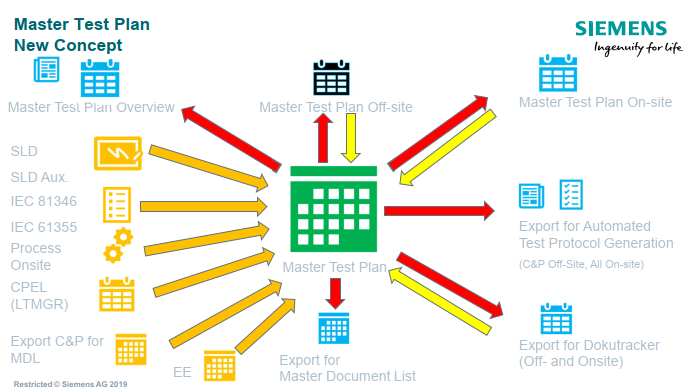
\includegraphics[width=0.9\textwidth]{Bilder/mtp} 
   \caption{Konzept des MTP, \cite{9}(S.2)} 
   \label{fig:struktur} 
   \end{center}
\end{figure}
%%
Er dient als Informationsursprung für weitere Dokumente und Arbeitsschritte im Laufe der Projektabwicklung. Durch Importe aus Listen und Diagrammen, die vom Kunden zur Verfügung gestellt werden, soll die Basis des \ac{mtp} erzeugt  werden. Einige dieser Dokumente sind auch bei Abnahme der Anlage oder bei Auswahl der Bauteile dem Kunden vorzulegen.
%%
\subsection{Master Test Matrix}
\label{sub:mtm}
%%
Die \ac{mtm} beschreibt verschiedene Testfälle und Testbedingungen, welchen die Anlage sowohl on- als auch off-site unterzogen wird. 
Diese Systemtests der Anlage werden auch im \ac{mtp} dokumentiert.
%%
\section{Dokumentationsnormen IEC 61355, IEC 81346 und ihre Verwendung}
\label{sec:iec}
%%
Da genannte Normen äußerst umfangreich und tiefgreifend sind, aber nicht alle Informationen zum Bearbeiten des Themas benötigt werden, wird im folgenden nur auf die wichtigen Grundlagen eingegangen.
Folgendes ist eine Zusammenfassung der relevanten Informatinen aus \cite[Kapitel 1-5]{3}, \cite[Kapitel 1-5]{4}, \cite[Kapitel 1-4,6]{5} und Gedankenprotokollen aus Mitarbeitergesprächen.
Die Normen enthalten Aussagen und Regeln zur Klassifizierung von Objekten und Dokumentationen in Stationen für Verteilung und Übertragung elektrischer Energie. Gearbeitet wird grundsätzlich noch mit dem Stand der Normen aus dem Jahr 2009 (IEC 81346-1/2) bzw. 2008 (IEC 61355).
\subsection{IEC 81346}
\label{sub:81346}
Die Kennzeichnung nach IEC 81346 bietet gegenüber früher genormten Kennzeichnungen weitergehende Möglichkeiten mit entsprechendem Rationalisierungspotential.
In IEC 81346-1 kann nach Aspekten unterschieden werden, diese sind Produktaspekt, Ortsaspekt und Funktionsaspekt. Ein Aspekt beschreibt die Betrachtungsweise für das Objekt. Grundsätzlich sollte jedes Objekt nach Produktaspekt strukturiert werden. IEC 81346-1 strukturiert Objekte nach diesen Aspekten und lässt somit eine klare Anlagenzusammensetzung erkennen. 
IEC 81346-2 typisiert Objekte in unterschiedliche Klassen und Unterklassen. Diese kommen auch bei der Strukturierung zum Einsatz.
In \ac{hgü}-Projekten wird die Dokumentenkennezichnung nach obenstehenden Normen durchgeführt. Objektkennzeichen beschreibt im weiteren die Kennzeichnung nach IEC 81346-1 und IEC 81346-2, zusammengesetzt aus Referenzkennzeichen und Objekttyp.
\\
\\
\subsubsection{Referenzkennzeichen}
\label{sub:refref}
%%
Das Referenzkennzeichen besteht aus maximal acht Leveln, beginnend mit der Stationsnummer. Danach folgt optional eine \markss{tieferliegende} Komponente. 
Die Strukturierung erfolgt meist von oben nach unten (top-down) oder von unten nach oben (bottom-up). Die Regeln erlauben im Prinzip einen Wechsel des Aspekts zwischen den Untergliederungsstufen einer Struktur, was jedoch in der Praxis selten zur Anwendung kommt.
%%
\begin{figure}[H]
   \begin{center}
   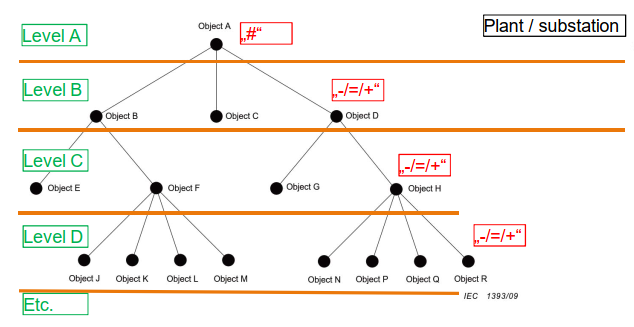
\includegraphics[width=0.9\textwidth]{Bilder/produktstruktur} 
   \caption{Struktur, \cite{10}(S.10)} 
   \label{fig:struktur} 
   \end{center}
\end{figure}
%%
Level A bezeichnet immer die Station, Level B und weitere beschreiben je eine durch einen Kennbuchstaben zugeordnete Funktion. Die Kennbuchstaben sind in der Norm tabellarisch festgehalten.
Einige Kennbuchstaben haben zusätzliche Unterklassen, um die Funkttion zu präzisieren. Sie werden durch zweistellige Kennbuchstaben definiert.
Die Kennbuchstaben der Strukturebene B und C sowie Darunterliegende unterscheiden sich grundsätzlich. Level B beschreibt Infrastrukturklassen, wie z.B. Umspannanlagen durch den Kennbuchstaben \markss{T}, während Level C und alle darunter Liegenden eine Klassifizierung nach Zweck oder Aufgabe beschreiben, z.B. definiert \markss{KF} die Funktion \markss{Verarbeiteung von elektrischen und elektronischen Signalen}.  
Der Übergang in das nächst niedrigere Level wird durch ein Trennzeichen dargestellt . Bei einem Funktionssaspekt wäre der Seperator \markss{=}, bei einem Ortsaspekt \markss{+} und bei einem Produktaspekt \markss{-}.
Erlaubt ist jedoch auch die Schreibweise \markss{-A1B1C1} oder \markss{-A1.B1.C1} statt \markss{-A1-B1-C1}.\\
Normalerweise wird jedes Objekt bei Siemens angesichts des Produktaspekt strukturiert. \\
Jedes Referenzkennzeichen ist laut Norm einzigartig.
\newpage
%%
\subsubsection{Objekttyp}
\label{sub:objektt}
%%
Der Objekttyp bedient sich den selben Objektklassen wie Strukturevel C des Referenzkennzeichens.\\
\markss{Alle Objekttypen, die bei “Transmission Systems” verwendet werden, sind im \ac{otc} enthalten.} \cite{5}(S.16) \\
Intern wird das Kürzel \ac{otc} stellvertretend für die Objektklasse verwendet, ist vom OTC die Rede ist eigentlich die Objektklasse mit allen fünf Stellen gemeint.
Alle Objekttypen sind wie folgt aufgebaut.
%%
\begin{figure}[H]
   \begin{center}
   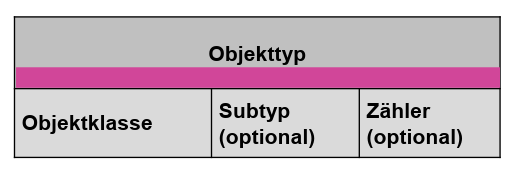
\includegraphics[width=0.9\textwidth]{Bilder/objekttypaufbau} 
   \caption{Zusammensetzung des Objekttyps, \cite{5}(S.18)} 
   \label{fig:objekttypaufbau} 
   \end{center}
\end{figure}
%%


%%
Bei der Bildung des Objekttyps wird unterschieden in physikalische und nicht-physikalische Objekte. \\
Nicht-physikalische Objekte behandeln Dokumente die keinem Produkt und keinem Ort eindeutig zugeordnet sind oder übergeordnet der Gesamtanlage dienen. Das sind z.B. Studien oder Projektmanagmentdokumente. Nicht-physikalische Objekte werden nur durch den Objekttypen gekennzeichnet. Sie haben kein Referenzkennzeichen. Nicht-physikalische Objektklassen werden durch fünf Zahlen gebildet, während physikalische Objektklassen aus zwei Buchstaben gefolgt von drei Zahlen bestehen.\\
Nicht physikalische Objekte sind in aktueller Ausarbeitung noch duch Siemens definiert. Der Zahlencode der physikalischen Objekte wird ebenfalls durch Siemens definiert, die Norm gibt nur den Buchstabencode vor.
Die Buchstaben entsprechen wie oben genannt dem Objektklassen-Code aus IEC8136-2.\\
Man erkennt in untenstehender Grafik deutlich, dass die Betrachtung des Objektes durch anhängen von drei Zahlen spezifiert wird.\\
%%
\begin{figure}[H]
   \begin{center}
   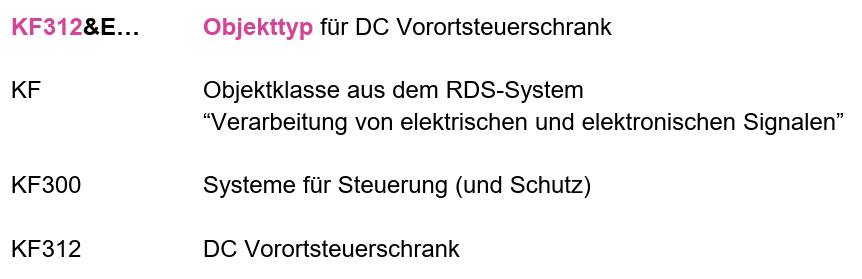
\includegraphics[width=1\textwidth]{Bilder/objekttyp} 
   \caption{Struktur eines physikalischen Objekttyps, \cite{5}(S.26)} 
   \label{fig:objekttyp} 
   \end{center}
\end{figure}
\newpage
%%
\subsubsection{Objektkennzeichen}
%%
Nachfolgende Grafik veranschaulicht die Kombination eines physikalischen Objekttyps und des Referenzkennzeichens nach Produktaspekt zum Objektkennzeichen.
%%
\pic{zusammen}{1}{Objektkennzeichen am Beispiel eines DC-Vorsteuerungsschrankes, \cite{5}(S.27)}{objektkennzeichen}
\newpage
%
\subsection{IEC 61355}
\label{sub:61355}
%
IEC 61355 erlaubt eine klar strukturierte Dokumentation zusammenhängend mit der eigenlichen Anlagenstruktur.
In der untenstehenden Grafik sieht man die Zusammensetzung der Normen zum Dokumentenkennzeichen bzw. Dokuemnetenseitenkennzeichen.
%%
\begin{figure}[H]
   \begin{center}
   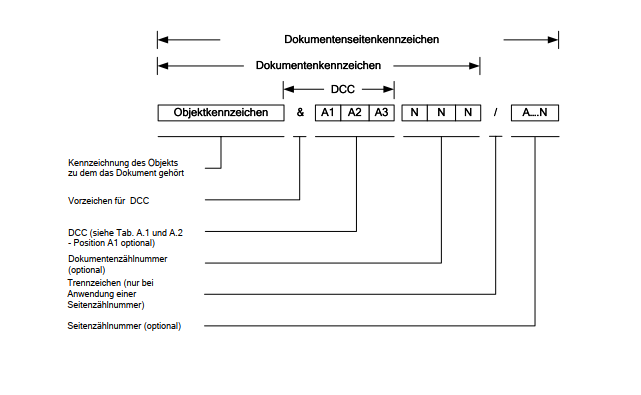
\includegraphics[width=1.1\textwidth]{Bilder/dokukennzeichen} 
   \caption{Dokumentenkennzeichnung, \cite{4}(S.12)} 
   \label{fig:dokk} 
   \end{center}
\end{figure}
%%
Wichtigster Bestandteil dieser Norm ist der \ac{dcc}.\\
Wie man in obiger Abbildung sieht, besteht der \ac{dcc} aus einem Vorzeichen, einem folgenden Kennbuchstaben, der den technischen Bereich des Dokuments bezeichnet und einem zweistelligen Buchstabencode, der die Dokumentenartklasse beschreibt. Die optionale Dokumentenzählnummer spezifiziert das Dokument. Der \ac{mtp} beinhaltet keinen \ac{dcc} ohne Dokumentenzählnummer. So beschreibt \markss{\&EFS010} einen dem Bereich Elektrotechnik (einschließlich Steuerungs-, Informations- und Kommunikationstechnik) zugeordneten Stromlaufplan. Das Kürzel \markss{FS} beschreibt übergeordnet Schaltkreisdokumente , während der Zahlencode \markss{010} auf Stromlaufplan spezifiziert.
Optional können noch Seitenzahlen angegeben werden.\\
Alle physischen Objekte, auch \markss{Equipment} genannt, bei Siemens folgen einer in \cite[S.47]{12} festgelegten Logik, nach welcher über jedes Objekt, übergeordnet eingteilt in Leittechnik- und nicht Leittechnik-Objekt, \markss{on-site} und \markss{off-site}, immer die selben Dokumentationen geführt werden müssen. Das komplette relevante Schema ist in Anhang \ref{sec:schema} zu sehen.
%%
\subsection{Dokumentennummer}
\label{sub:dokunummer}
%%
Die Anwendung beider Normen findet sich in der Bildung der Dokumentennummer wieder. Diese wird benötigt um alle Dokumente verschiedenster Art eindeutig zu kennzeichnen. Unter dieser Identifikationsummer werden diese später angelegt.
\\
%%
\begin{figure}[H]
   \begin{center}
   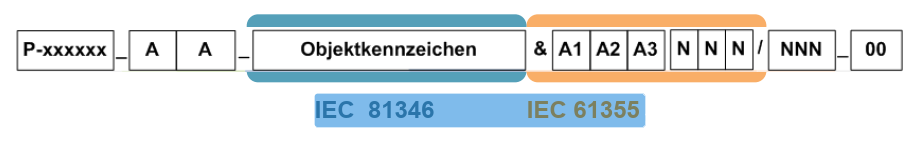
\includegraphics[width=0.9\textwidth]{Bilder/referenzkennzeichen} 
   \caption{Bildung der Dokumentennummer nach \cite{5}(S.8)} 
   \label{fig:doknum} 
   \end{center}
\end{figure}
%%

%%
Hinzu kommen hierbei noch der Projektcode, die zwei folgenden Kennbuchstaben und die Revisionsnummer an letzter Stelle. Der erste Kennbuchstabe beschreibt die Dokumentationsart, ob intern, extern oder Angebot, der zweite, den Aspektschlüssel aus Norm 81346-1.
\newpage
Der Aspektschlüsseltyp \markss{C}, der ein Objekt klassifiziert, das keinem anderen Aspektschlüssel zugewiesen werden kann, wird hier noch ergänzt. Das sind meist übergeordnete Dokumente zu mehreren Komponenten, z.B. Anlagenschaltpläne. Dieser ist nicht durch die Norm definiert, sondern intern. 
%%
\pic{aspectkey}{0.7}{Aspektschlüssel nach \cite{5}}{aspect}
%%
In der Grafik nicht sichtbar und auch in Norm bzw. interner Dokumentation nicht erwähnt, gliedert sich vor der Revisionsnummer noch das Sprachenkürzel für die Sprache des Dokuments ein.\\
Ein komplettes Beispiel einer Dokumentennummer ist \\
\inline{P-xxxxxx_EP_KF312#XY11-AF04-KF01-UH02&EFS010_EN_00}.
%%
\subsection{Dokumentendateiname}
\label{sub:dokudatei}
%%
Das Ablegen der Dokumente in den Projektverzeichnissen erfolgt durch einen der Dokumentennummer ähnlichen Dateinamen. Dieser wird aus der Dokumentennummer erzeugt, indem alle Trennzeichen durch \markss{\_} ersetzt werden. \markss{-}, \markss{+} und \markss{=} entfallen. Dadurch wird das Referenzkennzeichen als Block zusammengefasst. Die einzige Ausnahme besteht darin, dass das \markss{-} nach der Stationskennung zu einem \markss{\_} umgewandelt wird.\\
So ergibt sich \\
\inline{P-xxxxx_EP_KF312_XY11_AF04KF01UH02_EFS010_EN_00}.
%%
\newpage
\section{Polarion}
\label{sec:polarion}
%%
Wie einleitend genannt handelt es sich bei Polarion um ein browserbasiertes Tool, das Anforderungs-, Test- und Application-Lifecycle-Management, kurz ALM, liefert. \cite[vgl.]{1} \\
\markss{Polarion wird von globalen Unternehmen in einer Vielzahl von Branchen eingesetzt, wie zum Beispiel im Automobilbau, in der Medizintechnik und in der Luft- und Raumfahrt. Kunden erzielen mit Polarion die für die Herstellung Ihrer Produkte nötige Agilität, Traceability und Compliance. [...] Mehr als 2,5 Millionen Anwender weltweit vertrauen deswegen auf Polarion um die Zusammenarbeit in ihren Unternehmen voranzutreiben, ALM und Product Lifecycle Management (PLM) zu verknüpfen und um ihre hochwertigen Produkte auf den Markt zu bringen.} \cite{1} \\
Polarion läuft zentral auf einem Server, auf die der User per Browser zugreifen kann. \\
Die wichtigsten Funktion, die zur Implementierung dieser Arbeit dienen, werden folgend genannt. 
%%
\newpage
\subsection{Grundlegende Funktionalität}
\label{sub:funkti}
%%
In Polarion ist es möglich sogenannte Workitems einzupflegen, die an sich ein Objekt beschreiben. Dieses Objekt kann verschiedene Typen haben, dabei gibt es bereits fertige Standardtypen oder eigens erstellte \markss{Custom-Types}. Das Userinterface eines jeden Workitem-Types lässt sich durch erstellen neuer Felder bzw. das Umplatzieren dieser beliebig anpassen. 
Die in der Grafik erkennbare Kennung \markss{workitem-502} ist eine von Polarion selbst erzeugte ID, um jedes angelegte Workitem eindeutig zu kennzeichnen. Ein Ausschnitt der ganzen Benutzeroberfläche von Polarion ist im Anhang \ref{sec:polarionui} zu sehen. Darauf sieht man zusätzlich zur Grafik unten, noch das Fenster, in dem alle Workitems eines Typen aufgelistet werden. Diese Auflistung kann durch Abfragen verschiedener Parameter (Bilden von \markss{Queries}) manipuliert werden. Im Prinzip werden durch eine Query alle Workitems gefiltert und nach bestimmten Kriterien, z.B. dem Inhalt eines Feldes, gelistet. Die Poalrion-Query-Sprache ist grundsätzlich ähnlich zur Apache Lucene Syntax. \cite{13}
%%
\pic{testcase}{1}{Beispiel des Userinterface am Typen \markss{Test Case}}{testcase}
%%
Einige Felder des \ac{ui} sind bereits vordefiniert, meist werden sie vom System ausgefüllt, wie zum Beispiel das Feld \markss{Author}, und per default wie in Abbildung \ref{fig:testcase} zu sehen positionieren. Andere, sogenannte \markss{Custom-Fields} lassen sich per \ac{xml}-Datei anlegen und in einer auch als XML vorliegenden \markss{Form-Configuartion} im Interface anordnen. Es gibt viele unterschiedliche Custom-Field-Types, die häufigsten sind jedoch Enumeration und String.
\\
%%
\begin{figure}[H]
\begin{lstlisting}[language=XML]
<fields>
	<field description="Workitem Type" id="type" name="Type" type="enum:type"/>
	<field id="severity" name="Severity" type="enum:severity"/>
	<field id="author" name="Author" required="true" type="string"/>
	<field id="project" name="Project" type="string"/>
	<field id="categories" name="Categories" type="string"/>
<\fields>
\end{lstlisting}
\caption{Beispiel des Fields XML-Schema}
\label{fig:schema}
\end{figure} 
%%
Jede Felddefinition wird mit \inline{<field} begonnen und endet mit \inline{/>}. \inline{description} bezeichnet den in einer Pop-Up Box sichtbaren Text, wenn die Maus im UI über den Anzeigenamen des Feldes bewegt wird. \inline{name} beschreibt den Anzeigenamen des Feldes, \markss{id} den \ac{id} des Feldes und \inline{type} den Feldtypen.
Mit \inline{required="true"} wird festgelegt, welche Felder beim Anlegen eines einzelnen Items ausgefüllt sein müssen. Mit \inline{multi="true"} ist es möglich bei Feldern vom Typen \inline{enum} mehrere Optionen anzugeben.
Der Block der einzelnen Felder wird mit \inline{<fields>} begonnen und mit \inline{</fields>} beendet.
\newpage
%%
\begin{figure}[H]
\begin{lstlisting}[language=XML]
<!-- Horizontal layout element, adds components on horizontal row. Each component is in a new column. -->
    <horizontal>
        <!-- Vertical layout element adds components into one vertical column. Each component is in a new row. -->
        <vertical>
            <section>
                <field id="type" readOnly ="true" />
                <field id="severity" />
                <field id="author" />
                <field id="project" />
                <field id="categories" />
            </section>
 		  </vertical>
 	  </horizontal>
\end{lstlisting}
\caption{Beispiel des Form-Konfiguartion XML-Schema}
\label{fig:form}
\end{figure} 
%%
Wie im Beispielcode zu sehen beginnt \inline{<horizontal>} eine Reihe, \inline{<vertical>} eine Spalte und \inline{<section>} ein Element dieser Spalte. Wird ein Feld ohne Section definiert, so erscheint es als blauer Balken, wie \inline{Description} in Grafik \ref{fig:testcase}. 
Es gibt die Möglichkeit Felder mit \inline{readOnly="true"} nur lesbar zu setzen.
%%
Wenn ein Custom-Field als \markss{enum} definiert wird, muss in einem weiteren XML-Schema die Enumeration definiert werden. Enumerationen werden dann gewählt, wenn der Benutzer aus einem dropdown Listenfeld vorgegebene Werte auswählen soll. \\
%%
\begin{figure}[H]
\begin{lstlisting}[language=XML]
<enumeration>
	<option id="blocker" name="Blocker" description="" sortOrder="1"/>
	<option id="critical" name="Critical" description="" sortOrder="2"/>
	<option id="major" name="Major" description="" sortOrder="3"/>
	<option id="normal" name="Normal" description="" sortOrder="4" default="true"/>
	<option id="minor" name="Minor" description="" sortOrder="5"/>
	<option id="trivial" name="Trivial" description="" " sortOrder="6"/>
</enumeration>
\end{lstlisting}
\caption{Beispiel des Enumeration XML-Schema \markss{Severity}}
\label{fig:enum}
\end{figure} 
%%
Jeder auswählbare Wert wird hier als \inline{option} aufgeführt. Über den ID kann später darauf zugegriffen werden, \inline{name} gibt den Anzeigenamen an und \inline{description}, wie auch oben, den Text in der Pop-Up Box, die angezeigt wird, sobald die Maus über eine Option bewegt wird.
\inline{sortOrder} beschreibt die Reihenfolge in der die Optionen in der Klappliste angezeigt werden.
\\

Zusätzlich zu oben genannten Features verfügt Polarion über eine Import\-Funktion aus Excel-Workbooks und den Excel-Roundtrip-Change Import, bei dem bestehende Datensätze zuerst aus Polarion exportiert werden, bearbeitet und wieder importiert werden. Exportieren ist in fast alle gängigen Anzeigeformate möglich.\\
Verschiedene Benutzerrechtegruppen lassen sich auch erstellen.\\
Außerdem lassen sich in Polarion unterschiedlche Workitems miteinander verlinken, was es möglich macht Baumstrukturen zu erstellen, oder einen reinen Dokumentennamen mit dem tatsächlichen Dokument in Beziehung zu stellen.
\\
%%
%%
\subsection{Wiki Pages und Velocity}
\label{sub:veloc}
%%
Wiki-Pages sind editierbare Dokumente, die zum Anzeigen von Daten, Objekten und Informationen dienen sollen. Diese Dokumente stehen für jedes Projekt in einem übergeordneten Verzeichnis zur Verfügung. Sie sind Workitemtyp-unabhängig. Ein einfaches Beispiel hierfür wäre die Anzeige aller Workitems die mit einem bestimmten Flag, z.B. \markss{eilig} versehen sind. Diese \markss{Pages} können mit der Java-basierten Template Engine \markss{Velocity} (\cite{6}[vgl.]) editiert werden. Die verwendete Sprache, genannt \ac{vtl} lässt sich komplett in geschriebenen Text integrieren und bietet einige, wenn auch eingeschränkte, Funktionalitäten.
Diese Sprache soll \markss{die einfachste, unkomplizierteste und sauberste Möglichkeit bieten, dynamische Inhalte in eine Webseite zu integrieren.} \cite{6}. \\
Zusätzlich dazu stehen einige Templates aus Polarion zur Verfügung, die die Anzeige von Datensätzen vereinfachen oder einfach nur die Möglichkeit bieten Bilder in die Wiki-Page zu integrieren.
\\
Ein Zugriff auf die Polarion \ac{api} ist über bereits in­s­tan­zi­ie­rte Objekte der Services möglich, die einen Einstiegspunkt in die API ermöglichen.\\
Polarion arbeitet nicht mit der aktuellsten Version der \ac{vtl}, sonder mit Version 1.4. \cite[vgl. S.8]{18}\\
Ein kurzes Code-Beispiel unter Verwendung der API befindet sich in Anhang \ref{sec:veloapi}.
 
%%
%%
\subsection{API}
\label{sub:api}
%%
Polarion verfügt über eine Java \ac{api}, mit der es möglich ist Workitems zu ändern, zu lesen und zu erstellen, Benutzer zu verwalten, nach Workitems zu filtern oder Projekte aufzulisten, nur um ein paar Funktionen zu nennen. Zur Verfügung stehen verschiedene Services, mit unterschiedlichen Funktionen, mit denen der Zugriff auf den Polarion Server ermöglicht wird. (\cite{17}[vgl.]) \\
Einige der wichtigsten sind laut \cite{17}(S.3):
\subsubsection{ISecurityService}
%%
Ein Einstiegspunkt für Authentifizierungs- und Autorisierungsaufgaben. Die Aufgabe dieses Services ist es, Benutzer zu verwalten, Rollen zu verteilen, Beziehungen und Rechte anzulegen.
%%
\subsubsection{ITrackerService}
%%
Dieser Service dient als Haupteinstiegspunkt um Workitems zu verwalten. Er ermöglicht das Suchen, Lesen, Erstellen, Modifizieren und das verlinken von Workitems.
%%
\subsubsection{ITransactionService}
%%
Durch diesen Service ist es möglich Änderungen am Repository persistent zu machen. 
%%
\subsubsection{IDataService}
%%
Mit diesem Service ist eine Verwaltung von Objekt-Historien möglich.
%%
\subsection{Extension FMC}
\label{sub:fmc}
%%
Informationen über die Funktionsweise des Plugins, wurden dessen öffentlich einsehbaren Quellcodes bzw. der Funktionsanleitung entnommen. (\cite{8})\\
Die zur Verfügung gestellten Server haben bereits eine Extension vorinstalliert, die es möglich macht eigens verfasste Skripte in JavaScript in den Polarion-Wokflow zu integrieren. In diesen kann eingeschränkt auf die API zugegriffen werden, es stehen nur Instanzen des aktuellen Workitems, des \markss{TrackerService} und eines Loggers zur Vefügung.\\
Das Plugin überschreibt die von Polarion aufgerufene \markss{invoke}-Funktion, falls der \markss{save}-Parameter gesetzt ist und lässt somit nach dem Speichern eines Workitems, das die \markss{invoke}-Funktion mit dem gesetzten \markss{save}-Parameter aufruft, die Ausführung von eigenem Code zu. Sobald die im Code verfügbare Variable \markss{returnvalue} über einen Inhalt verfügt, wird dem User eine Error-Message angezeigt, die diesen Inhalt darstellt. Das Speichern wird somit verhindert. \\
Ein einfaches Beispiel wäre z.B. eine Überprüfung auf das Einhalten eines Prozentsatzes. Eine Kombination aus drei Feldern soll einen Prozentsatz von 100\% ergeben, bei einer Ungleichheit zu 100\% soll ein Speichern nicht möglich sein.
%%
%%
\subsection{PAM}
\label{sub:pam}
%%
Folgende Informationen sind aus einem Gedächtnisprotokoll mit Hr. Paul-Heinz Esters. \ac{pam} ist ursprünglich konzipiert um Software automatisch aus Anlagen-Datensätzen zu generieren. In \ac{pam} sollen zukünftig alle anlagenbezogenen Daten, von Nenndaten bis zu den Referenzkennzeichen der Bauteile gesammelt werden. Statt \ac{pam} zur Parametrisierung von Software zu benutzen, wird \ac{pam} allerdings als Daten-Backbone verwendet. 
%%
\section{Stand der Technik}
\label{sec:stand}
%%
Aktuell werden die Datensätze des \ac{mtp} über eine Excel-Tabelle verwaltet. Auf ein bestehendes Template wird über verschiedene Informationszugänge von Hand der schlussendliche Datensatz aufgebaut. Dieser Ansatz ist zwar funktional, aber grundsätzlich unhandlich und ohne einsichtlichen Userworkflow. Zusätzlich ist kein ausreichender Schutz vor Datenverlust bei Mehrfachzugriff möglich. 
Zu Arbeiten mit Polarion gibt es aktuell ein Pilotprojekt, dass die \ac{mtm} behandelt, ähnlich wie der \ac{mtp} über Excel verwaltet wurde.




